
\documentclass{beamer}

\usetheme{Copenhagen}
\usepackage[normalem]{ulem}
\title{DSP Lab Presentation}
\subtitle{EE3025 - Independent Project}
\usepackage{graphicx}
\graphicspath{{./images/}}

\author{
S.Abdur Rahman Nawaz -  \
\texttt{EE18BTECH11052}
}
\institute{IIT HYDERABAD}
\date{June 12, 2021}

\AtBeginSubsection[]
{
  \begin{frame}<beamer>{Outline}
    \tableofcontents[currentsection,currentsubsection]
  \end{frame}
}

\begin{document}

\begin{frame}
  \titlepage
\end{frame}
\section{Problem Statement}

\begin{frame}[fragile]
\begin{itemize}
    \item{ Modify the following code given in problem 2.3 with different input parameters to get the best possible output.}
\end{itemize}
\begin{verbatim}
import soundfile as sf
from scipy import signal
    
input_signal,fs = sf.read('Sound_Noise.wav')

sampl_freq=fs
order = 3
cutoff_freq=4000.0
Wn=2*cutoff_freq/sampl_freq

b, a = signal.butter(order,Wn,'low')
output_signal = signal.filtfilt(b, a, input_signal)
sf.write('Sound_With_ReducedNoise.wav', output_signal, fs)
    
\end{verbatim}
\end{frame}

\section{Solution}

\begin{frame}{Solution}
  The main parameters for a standard Butterworth filter are, 
  \begin{itemize}
  \item{Cutoff frequency}
  \item{Order}
  \end{itemize}
\end{frame}

\begin{frame}{Solution}
  \textbf{Cutoff Frequency:} 
  
%   \subsection{\textbf{Cutoff Frequency}}
  Cutoff frequency for a Butterworth filter is the $-3dB$ point after which all the frequency components roll off down to zero.\\
  To select a good cutoff frequency, we observe the spectogram from Problem 2.2 and conclude that most of the frequencies corresponding to piano notes are around mid point of 440Hz and 4700Hz, so let the cutoff frequency be $(440+4700)/2 = 2570Hz$
  
% \section{\textbf{Results}}
%     After applying the filter with above parameters we observe that we still have noise. The frequency response of signal before and after applying the filter shows that the transition region is too wide, there are too many non zero frequency components after the cutoff frequency.
\end{frame}

\begin{frame}{Solution}

  \textbf{Order:} 

%   \subsection{\textbf{Order}}
  The main disadvantage of the Butterworth filter is that it achieves the pass band flatness at the expense of a wide transition band as the filter changes from the pass band to the stop band.\\
  We can fix this by increasing the order, but having a very high order would create numerical instabilities while simulating. So we will stick to the general order 4.
\end{frame}


\begin{frame}{Solution}
\textbf{Results:}
    After applying the filter with above parameters we observe that we still have noise. The frequency response of signal before and after applying the filter shows that the transition region is too wide, there are too many non zero frequency components after the cutoff frequency. \\
  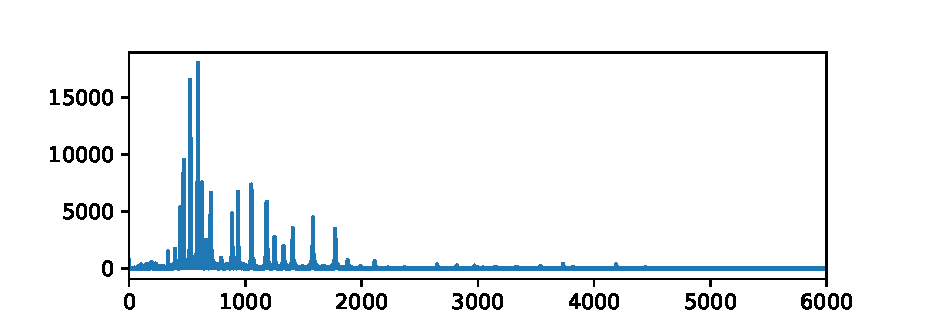
\includegraphics[scale =0.35]{./figures/before.eps} 
  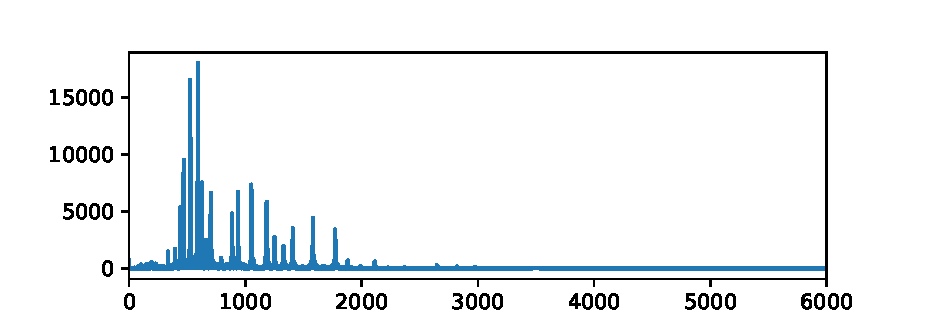
\includegraphics[scale =0.35]{./figures/after-1.eps} 
  .\hspace{1cm} Before Filtering \hspace{3cm}     After Filtering
\end{frame}


\begin{frame}{Solution}

    To overcome this we would need a steeper transition. Since we cant increase the order, one solution is to cascade multiple butterworth filters. The transfer function rolls off to zero from pass band to stop band, as we cascade more and more filters the gain values$<1$ would get multiplied and reach closer to zero.
    \begin{center}
        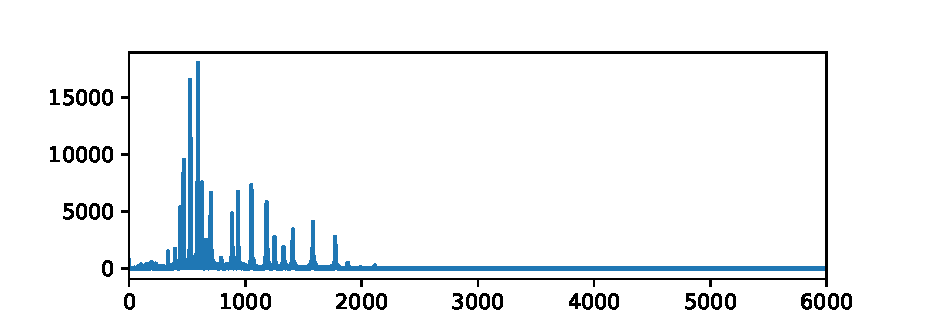
\includegraphics[scale =0.5]{./figures/after-2.eps} 
    \end{center}
    .\hspace{3cm} After Cascaded Filtering
\end{frame}

\begin{frame}{Solution}
To get a better understanding of the noise present in the signal we sum up all the non zero frequency
components before and after the cutoff frequency to define the metric fraction which tells us how much non zero frequency component is present before and after the cutoff.
    \begin{center}
        \begin{tabular}{ |c|c|c|c| } 
             \hline
             Parameter & Original & Filtered & Cascaded\\
             \hline
             Cutoff Frequency & $2570Hz$ & $2570 Hz$ & $2570 Hz$\\ 
             \hline
             Order & - & 4 & 4 \\ 
             \hline
            No. of Cascades & - & 0 & 19 \\ 
             \hline
            Fraction of signal & 82.35\% & 97.38\% &  99.51\%\\
            before cutoff & & &\\
            \hline
            Fraction of signal  & 17.64\% & 2.61\%  & 0.485\%\\
            after cutoff & & &\\
            \hline
        \end{tabular}
    \end{center}
\end{frame}

\section{Appendix}
\begin{frame}{Appendix}
    \begin{itemize}
        \item{C code for generating the plots with FFT and IFFT implementations can be found
        \href{https://github.com/AbdurNawaz/EE3025/tree/main/Assignment-1/codes}{\uline{here}}.}
        \item{Python codes for generating the plots can be found \href{https://github.com/AbdurNawaz/EE3025/tree/main/Assignment-1/codes}{\uline{here}}.}
        \item{Input and Output Sound files can be found \href{https://github.com/AbdurNawaz/EE3025/tree/main/Assignment-1/soundfiles}{\uline{here}}.}
    \end{itemize}
    
\end{frame}
\end{document}

